% Note when we get to this section we can introduce temporal variation by stretching or shrinking our signals to augment our dataset to get more samples (and simulate potential an older adult).

\section{Selecting Cooking Tasks}
To employ some of the time-series classification methods discussed in Chapter \ref{chp4}, a dataset of the proposed positional + IMU system is required. Chapter \ref{chp2}'s section on the traditional assessments of ADLs will serve as a basis for the selection of tasks to perform and collect data from. Of the assessments discussed, Table \ref{tab:cooking-task-summary} summarizes the assessments with cooking tasks mentioned in its procedure.

\begin{table}[ht]
    \small
    \centering
    \caption{Cooking tasks in the Assessment tools for the IADLs.}
    \label{tab:cooking-task-summary}
    \renewcommand{\arraystretch}{1.5}
    \begin{tabularx}{\textwidth}{>{\hsize=.8\hsize}X X }
        \hline
        \textbf{Tool} & \textbf{Tasks} \\
        \hline
        PASS & making soup with water/milk \\
        & making muffins in the oven \\
        & cutting up fruit \\
        Self-Assessment PD Disability Scale & making a cup of tea \\
        & inserting electrical plug \\
        & pouring milk from bottle \\
        & opening tins \\
        & washing \\
        Melbourne Low-vision ADL Index & preparing meals \\
        Lawton Instrumental ADL Scale & plans, prepares and serves adequate meals independently \\
        Frenchay Activities Index & preparing main meals \\
        Texas Functional Living Scale & Describe how to make peanut butter and jelly sandwich \\
        \hline
    \end{tabularx}
\end{table}

Of the assessments in Table \ref{tab:cooking-task-summary}, the cooking task(s) in the Melbourne Low-vision ADL Index, Lawton Instrumental ADL Scale, Frenchay Activities Index, and Self-Assessment PD Disability Scale are all questionnaires and as a result do not have concrete steps on how the task should be performed. Futhermore, the Melbourne Low-vision ADL Index, Lawnton Instrumental ADL Scale and the Frenchay Activities Index only have general requirements for the cooking task such as the ability to "prepare meals," and "plans, prepares and serves adequate meals independently." These general cooking tasks may be useful in the evaluation of ADL ability in a questionnaire format by requesting the older adult to holistically consider their ability to cook, but may not be the best candidates when looking for fine-grained actions to extract. 

The remaining 2 assessment tools, the Texas Functional Living Scale and Performance Assessment of Self-Care Skills (PASS), mention cooking task(s) that requires a clinician to evaluate. Upon closer inspection of the Texas Functional Living Scale, however, the individual is only required to describe the task and not actually perform it. The only candidate that has clear cooking tasks broken down into their fine-grained actions is the PASS and will be used as a reference for the experiment protocol and extraction of fine-grained tasks. 3 Cooking Scenarios are presented in the PASS: making soup with water/milk, making muffins in the oven, and cutting up fruit. The 3 cooking scenarios are shown in Figures \ref{fig:PASS-muffin}-\ref{fig:PASS-soup}.

\begin{figure}[ht]
    \centering
    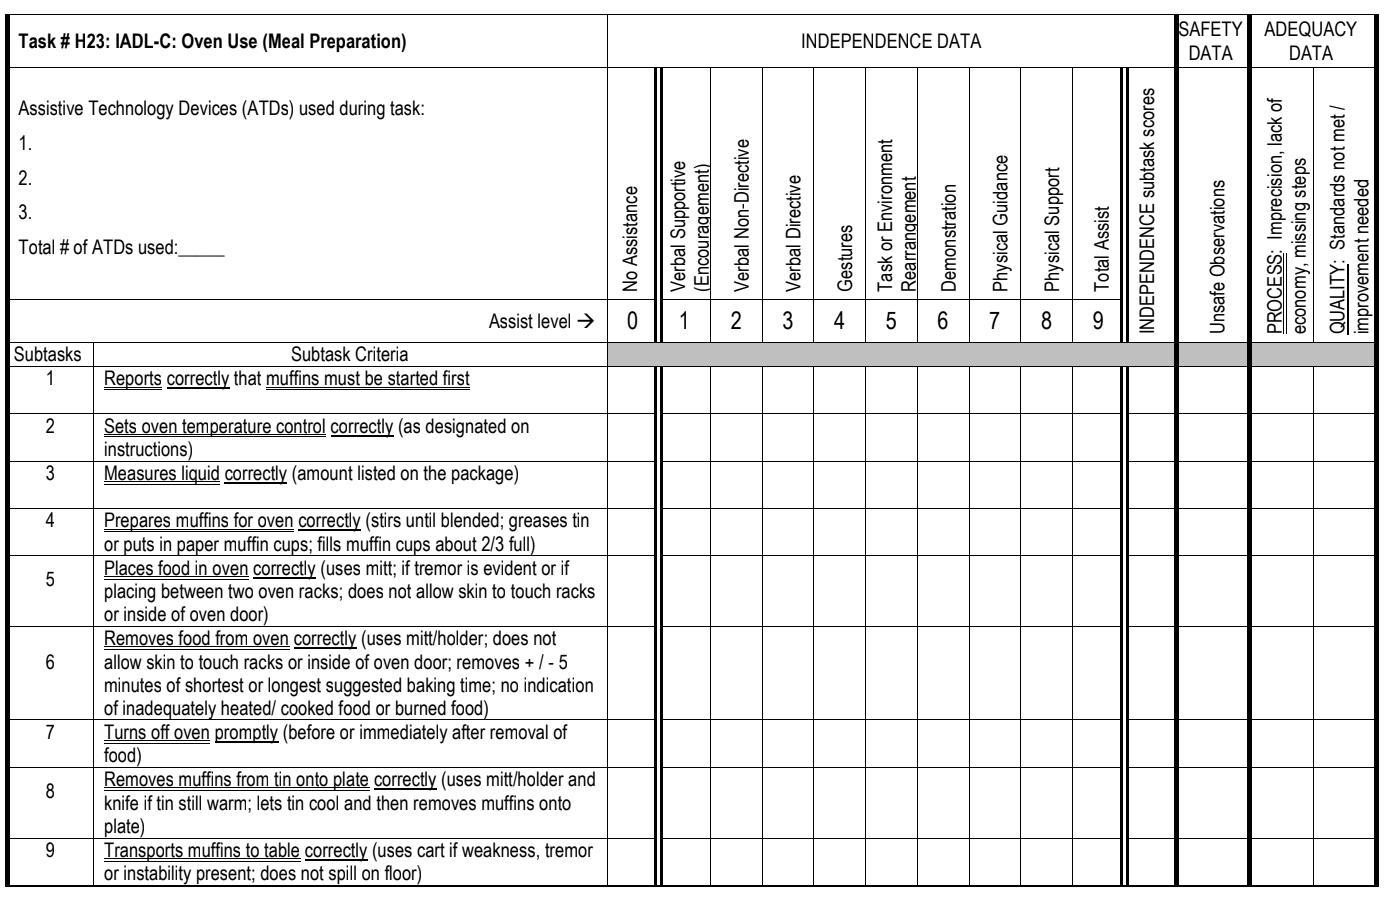
\includegraphics[width=0.95\textwidth]{pass-muffin.png}
    \caption{PASS Muffin Task \cite{rogers_performance_2014}}
    \label{fig:PASS-muffin}
\end{figure}


\begin{figure}[ht]
    \centering
    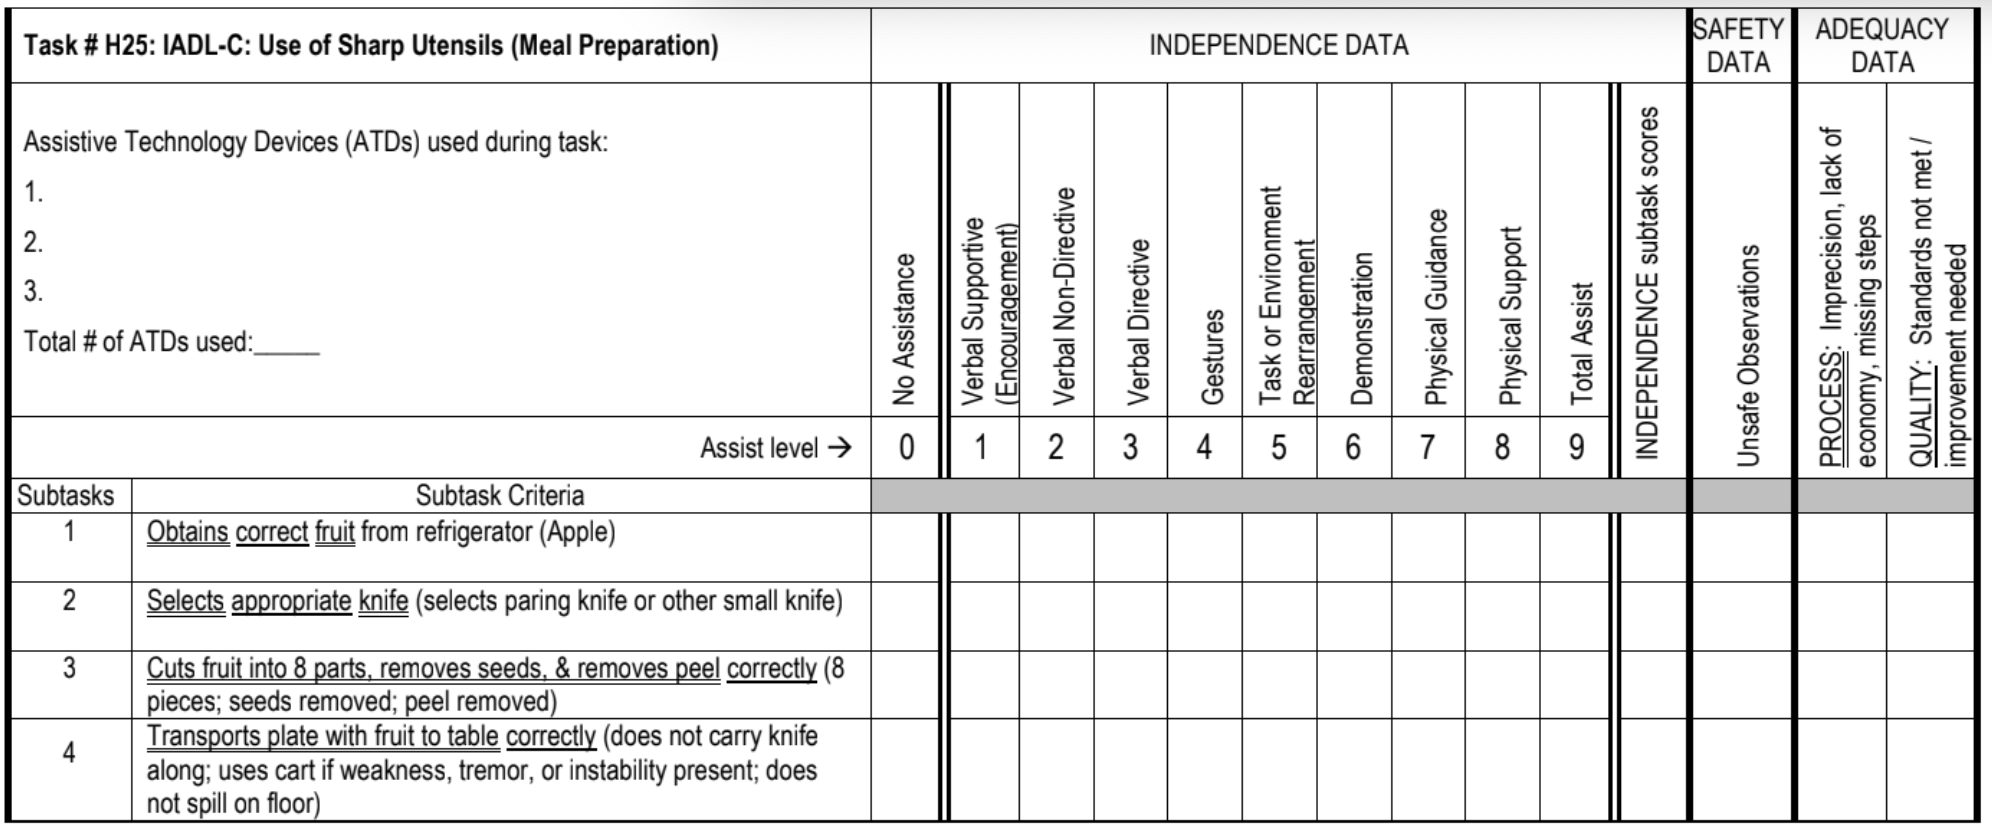
\includegraphics[width=0.95\textwidth]{pass-fruit.png}
    \caption{PASS Fruit Task \cite{rogers_performance_2014}}
    \label{fig:PASS-fruit}
\end{figure}

\begin{figure}[ht]
    \centering
    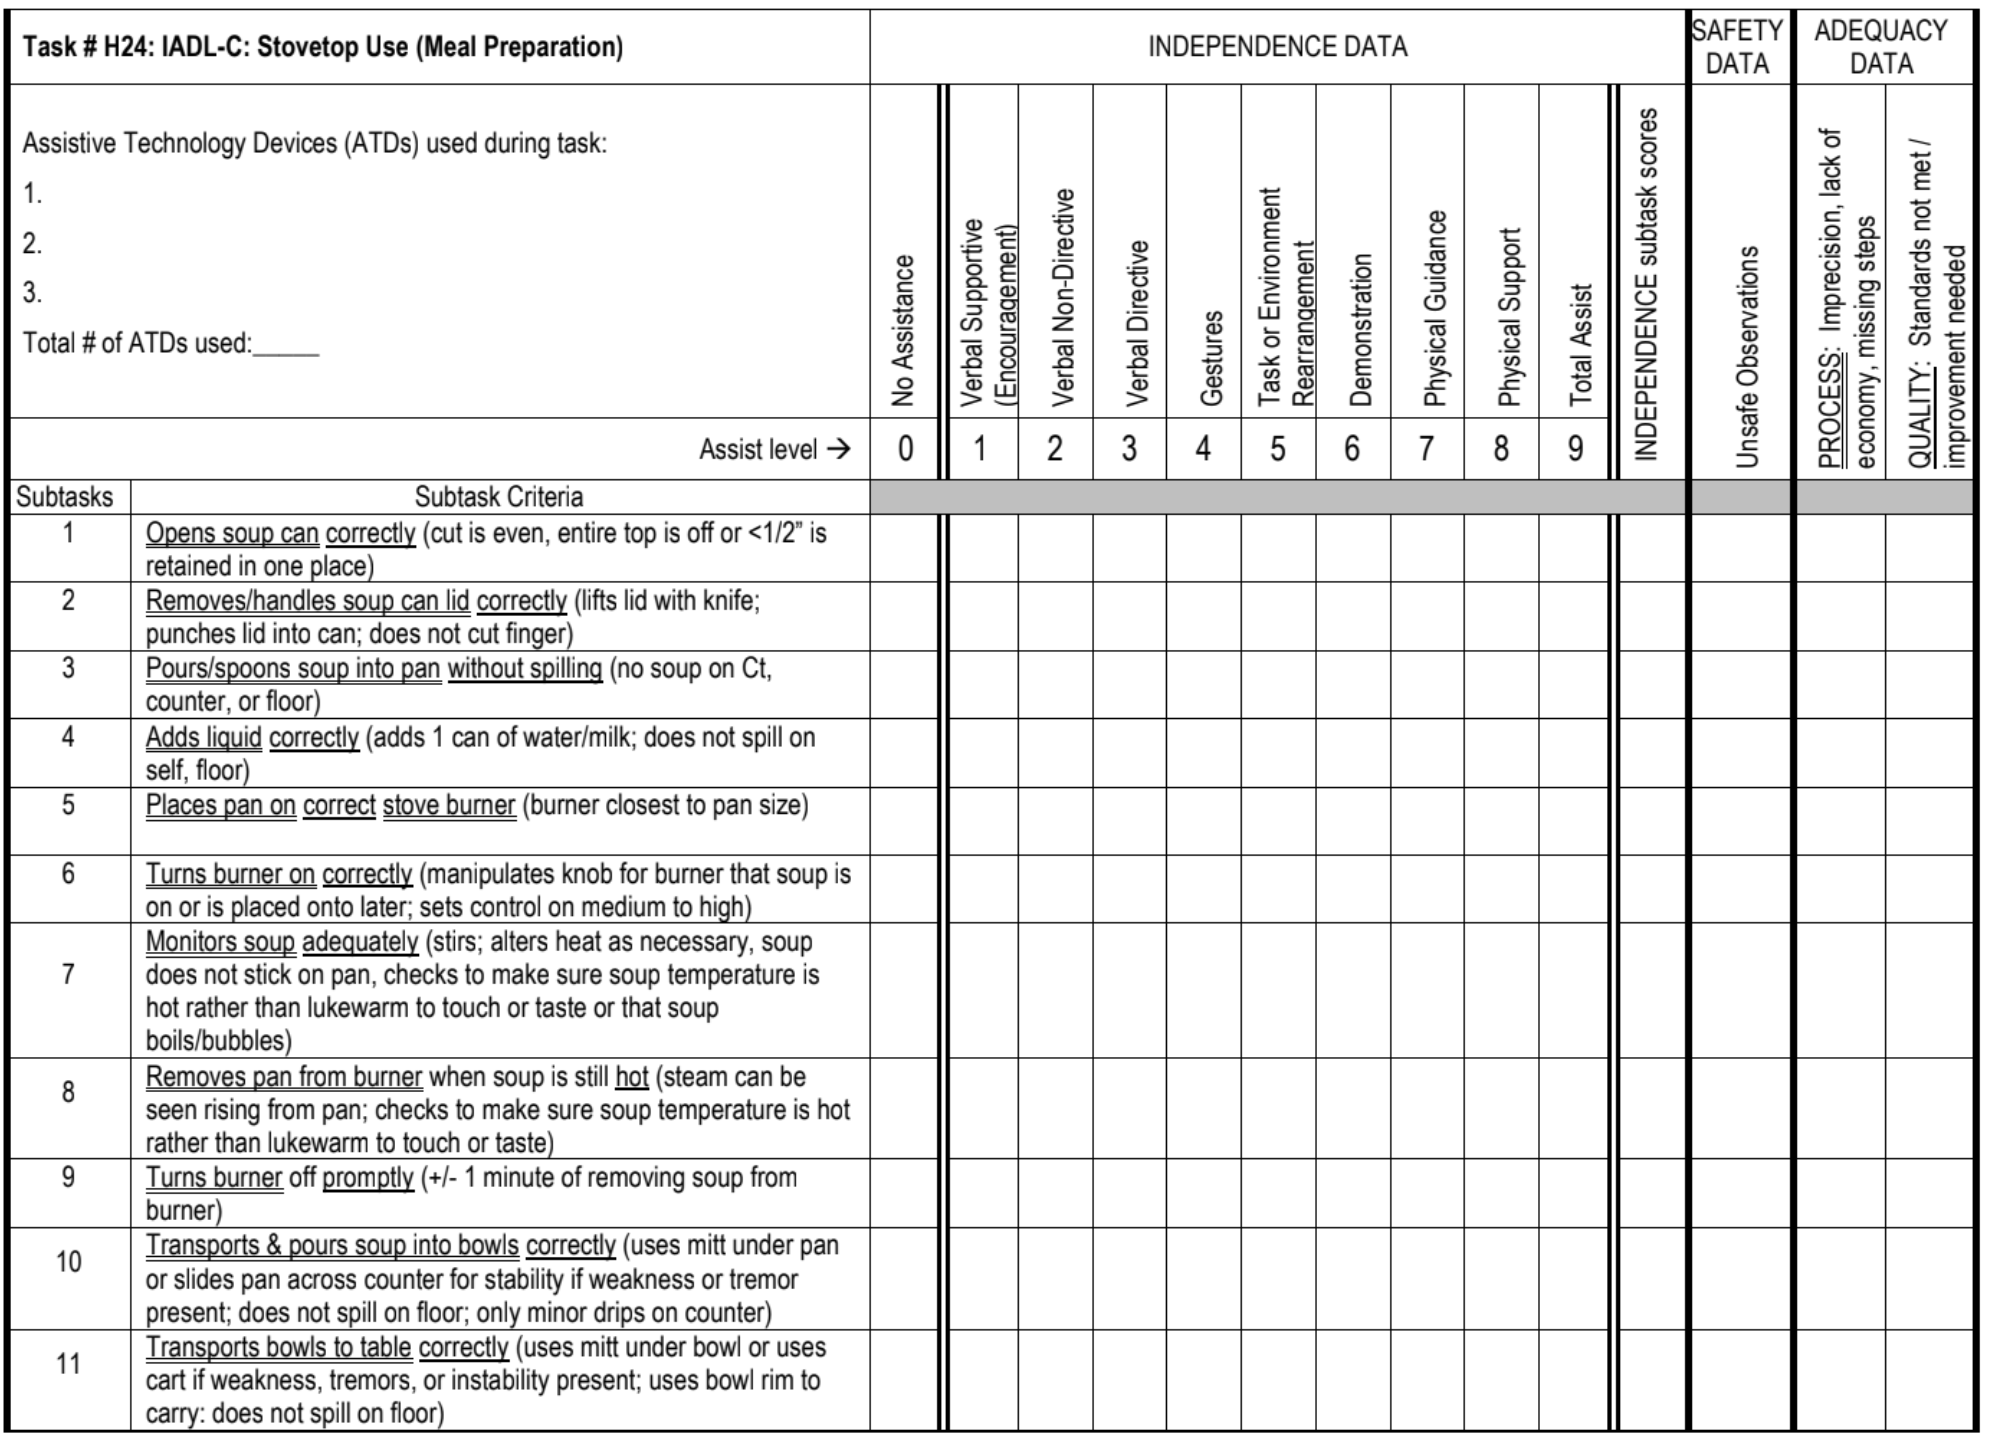
\includegraphics[width=0.95\textwidth]{pass-soup.png}
    \caption{PASS Soup Task \cite{rogers_performance_2014}}
    \label{fig:PASS-soup}
\end{figure}

\section{Fine-grained Task Extraction}
The detail in which tasks can be broken down varies in literature. Human actions may be decomposed all the way into action primitives which is a body part + some motion (eg. right/left hand forward/backward) \cite{huszHumanActivityRecognition2007}. Fine-grained actions can be thought as being one level "coarser" than these action primitives and may combine action primitives to perform a small task (eg. cutting fruit, stir-frying, washing a fruit)  \cite{pan_fine-grained_2020}. A "coarser" level above fine-grained actions are coarse-grained actions and describe the activity that encompasses all of the fine-grained actions (eg. cooking, working). Although action primitives may be useful to consider when breaking down a task, the focus of the thesis is the evaluation of function and ability to perform tasks toward some goal. The detection of coarse-grained actions or activities have been successful in literature previously \cite{cook_learning_2010}, but these coarse-grained actions are too general and do not provide insight into the functional quality of the cooking task. Thus, the focus of the task extraction will be at the "fine-grained" level. 

For each cooking activity in the PASS, an experimental protocol will be developed based on the subtasks outlined in the task document. Although the PASS presents general steps to complete the task, there may sometimes be other actions, or "side-actions" involved in the task. For example, for the Cutting Fruit task in Figure \ref{fig:PASS-fruit}, obtaining the fruit from the refrigerator would require the individual to perform OPEN\_FRIDGE, GRAB\_FRIDGE, and CLOSE\_FRIDGE. The experimental protocol will be more detailed with steps detailing the actions in the PASS as well as any side-actions that occur. Then, from the steps in the experimental protocol, the fine-grained actions can be extracted.



